%!TEX program = xelatex
%This script will not compile using pdflatex
%Uses the Beamer M Theme, copyright Matthias Vogelgesang
%This can be found at https://github.com/matze/mtheme
\documentclass[10pt, compress]{beamer}
\usetheme[titleprogressbar]{m}

\usepackage{booktabs}
\usepackage{amsmath}
\usepackage{amssymb}

\title{Beyond Friendship and Followers: The Wikipedia Social Network}
\subtitle{}
\author{Johanna Geiss, Andreas 	Spitz, Micheal Gertz}
\institute{Vaibhav Sinha, Vishwak S., Chandra Kiran Evuru\\
\texttt{CS15BTECH110\{34, 43, 12\}}}

\graphicspath{{images/}}

\begin{document}

\maketitle

\begin{frame}[fragile]
  \frametitle{Introduction}
\begin{itemize}
  \item \textbf{Goal:} Extract a large-scale person-centric network structure form English Wikipedia.
  \item Persons mentioned on a Wikipedia page have a common context, closer the names more evident the relationship.
  \item Wikidata contains data about 1.2M persons.
  \item Extracting persons based on IWL and drawing edges based on co-occurrences and distance, obtain a person network of roughly 800k persons and 67M edges.
  \item Identify centrality, clustering coefficients and component sizes.
  \item Also identify interesting communities and evaluate them .
  
\end{itemize}
\normalsize
\end{frame}

\begin{frame}[fragile]
  \frametitle{Related Work}
\begin{itemize}
\item Most approaches for extracting person-centric and social networks for academics from semi-structured data such as documents and web pages concentrate on co-authorship and academic collaborations, because author names mostly co-occur and appear with metadata.
\item Networks have been extracted from mail archives and blogs.
\item Approaches have been attempted to recover the social graph from Wikipedia but none attempts to create directly from wikipedia pages.
\item Creation of graphs based on co-occurances of names from web pages have been attempted but the method of extract the names have not been very generalizable.
\end{itemize}
\tiny
\normalsize
\end{frame}

\begin{frame}[fragile]
	\frametitle{Extracting person information from Wikipedia (WP)}
\begin{itemize}
\item WP has more than 16.8M items. \footnote{As on January 26, 2015}
\item Wikidata (WD) classifies 2.6M entries from WP as instances of humans, 45\% ($\sim$1.2M) of which are English.
\item Gender ratio: 84.3\% male, 15.6\% female, 0.1\% other or unknown 
\item 83, 75\% have date of birth and death.
\end{itemize}
\begin{figure}
  \centering
 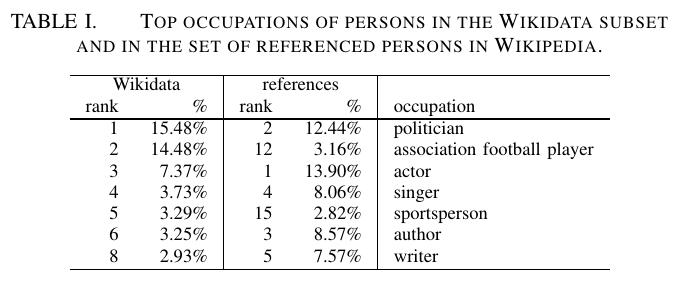
\includegraphics[width=7cm,height=3cm]{Table1.png}
\end{figure}
\end{frame}

\begin{frame}[fragile]
	\frametitle{Recognition of persons in Wikipedia}
\begin{itemize}
\item WP contains 5.29M content pages, about 65M sentences. \footnote{As on January 12, 2015}
\item Classify a WP page as a person page based on year of birth and death, results in 1.05M pages.
\item The count is lesser than (by 178,807) WD owing to the heuristic used and difference in the creation date.
\item To find references to persons in all Wikipedia page, a two step process is used, first following IWLs and then searching for 	recognized person names.
\end{itemize}
\end{frame}

\begin{frame}[fragile]
	\frametitle{Following interwiki links (IWLs)}
IWL is of the form [[\textit{linkTarget}|\textit{coveredText}]], where \textit{coveredText} is optional.
\begin{figure}
  \centering
 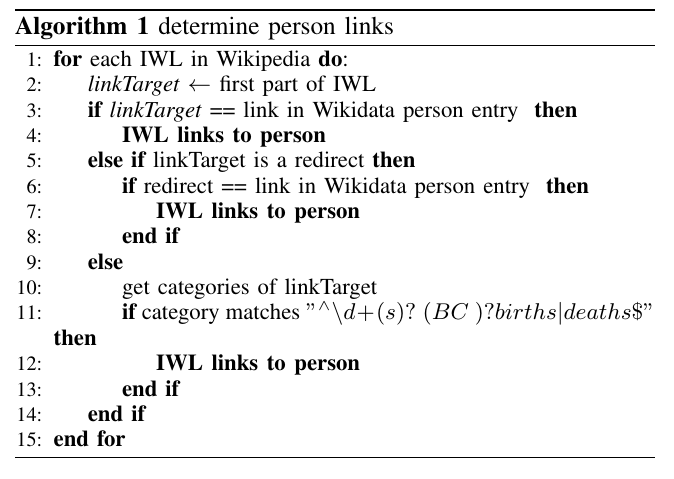
\includegraphics[width=7cm,height=5cm]{Algo1.png}
\end{figure}
\end{frame}

\begin{frame}[fragile]
	\frametitle{Following interwiki links (Cont.)}
\begin{itemize}
\item English WP has 76.8M IWLs of which 13.6\% ($\sim$10.4M) refer to persons.
\item 99.9\% of these are identified by WD.
\item Each person is labeled using an ID either from WD or WP.
\item About a third of the content pages in WP have IWLs to persons.
\item The person-IWLs refer to 842,484 persons, 99.6\% of which are in WD.
\end{itemize}
\begin{figure}
  \centering
 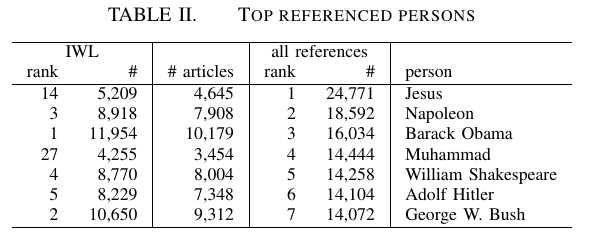
\includegraphics[width=6cm,height=2.5cm]{Table2.png}
\end{figure}
\end{frame}

\begin{frame}[fragile]
	\frametitle{Searching for recognized person names}
\begin{itemize}
\item Search each page for persons that are already referred to in an IWL on that page.
\item About a third of pages that link to a person page also contain references to persons outside IWLs.
\item A total 2.7M references to 273K persons in 631K pages outside IWL's.
\item Combining both, a total of 13.14M mentions in 1.89M WP articles. 510K of these have only one IWL.
\item \textit{Rosters of the top basketball team in European Club competitions} has a highest 4,694 mentions of 1,761 persons.
\item \textit{List of Test cricketers} has a highest 2,685 persons.
\end{itemize}
\end{frame}

\begin{frame}[fragile]
	\frametitle{Recognition of persons in Wikipedia (Cont.)}
\begin{itemize}
\item 83.8\% IWLs link to male, 15.8\% to female.
\item 839,490 persons in WD are referenced in WP, 392,215 are either not referenced or referenced in untracked regions.
\end{itemize}
\begin{figure}
  \centering
 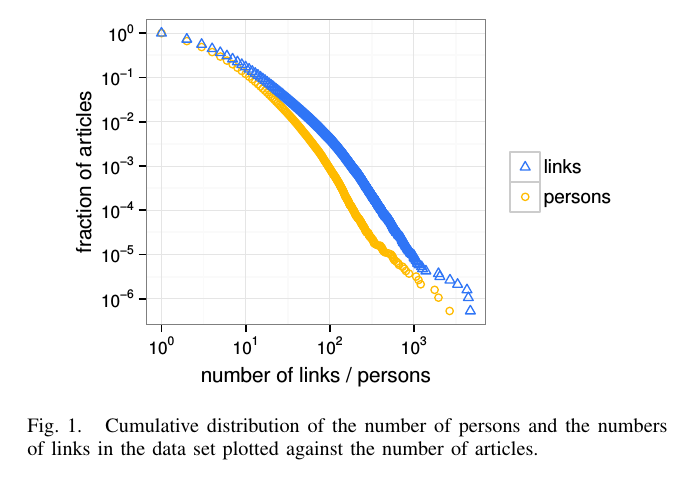
\includegraphics[width=7cm,height=5cm]{Fig1.png}
\end{figure}
\end{frame}

\begin{frame}[fragile]
	\frametitle{Person-Centric Network Construction}
\begin{itemize}
\item The network is represented in the form of a bipartite graph \(G = (V \cup D,E)\), where
\begin{itemize}
\item \(V\) : Set of nodes corresponding to people.
\item \(D\) : Set of nodes corresponding to the Wikipedia documents.
\item \(E\) : Set of edges \((u,p)\) such that \(u \in V\) and \(p \in D\) and iff document \(p\) contains person \(v\).
\end{itemize}
\item To construct a network of persons, we project graph \(G\) onto the set of persons.
\item We create a multi-graph as projection for each co-occurence between two persons as a single edge and then aggregate the edges to obtain a graph w/o multiple edges.
\end{itemize}
\end{frame}

\begin{frame}[fragile]
	\frametitle{Person-Centric Network Construction}
\begin{itemize}
\item Weights of edges in the multi-graph are given by : 
\begin{equation} \varphi(e = (v, w, i)) := e^{-d(v,w,i)/2} \end{equation}
\begin{itemize}
\item \(v,w\) : Belong to the set of persons.
\item \(i\) : Instance of a co-occurence between v and w 
\item \(d\) : Distance between v and w measured as the number of sentences between v and w in the documment that corresponds to i'th co-occurence.
\end{itemize}
\item To convert into a graph with single edges b/w two persons we aggregate multiple edges by cosine similarity of neighbourhoods for the two nodes.
\end{itemize}
\begin{equation}
dicos(v,w) = \frac{\sum_{e\in n_v \cap n_w} \varphi(e)^2}{\sqrt{\sum_{e\in n_v} \varphi(e)^2}\sqrt{\sum_{e\in n_w} \varphi(e)^2}}
\end{equation}
\end{frame}

\begin{frame}[fragile]
	\frametitle{Network Properties}
\begin{itemize}
\item The aggregated network contains exactly \(67, 583, 553\) edges, which connect the \(799, 181\) persons.
\item A large part of the graph \(\approx 98.8\%\) is contained in one giant component / cluster.
\item Such a large network will cause inefficient future-processing such as community detection or finding network centrality.
\begin{itemize}
	\item For this purpose, the authors have considered edge weight thresholding i.e., an original edge exists if the edge weight is greater than a particular threshold \(\zeta\),  to make the graph rather sparse.
    \item Using this sparser network, network centrality and community detection are run on them.
\end{itemize}
\end{itemize}
\end{frame}

\begin{frame}[fragile]
	\frametitle{What is my threshold for making a sparse graph?}
\vspace{-7mm}
\begin{itemize}
\item Following motivation from previous work by Freeman and Serrano \textit{et al}, the authors consider certain structural metrics of the graph for this purpose.
\item 5 structural metrics are taken into consideration:
\begin{itemize}
	\item Clustering Coefficient: A measure of the tendency of two nodes to cluster together. A global clustering coefficient defined by Luce and Perry can be mathematically defined as:
    \[cc = \frac{\mathrm{Number of closed triplets}}{\mathrm{Number of connected triplets of vertices}}\]
    \item Assortativity Coefficient: A measure of the tendency of two nodes in different networks to attach to each other. It is analogous to Pearson Correlation for vectors.
    \item Percentage of remaining edges: Once the threshold is set, certain edges will be deleted / removed.
    \item Average component size: The average size of the components of the graph for a given threshold
    \item Number of connected components
\end{itemize}
\end{itemize}
\end{frame}

\begin{frame}[fragile]
	\frametitle{What is my threshold for making a sparse graph? {\small (contd..)}}
\vspace{-5mm}
\begin{figure}
	\centering
    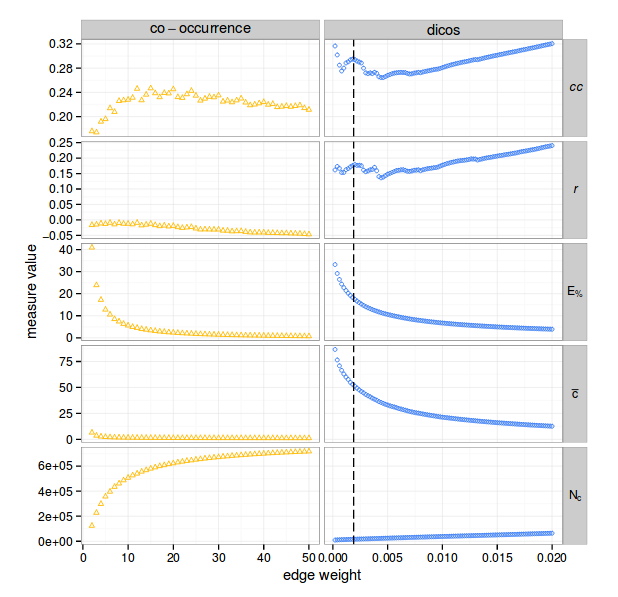
\includegraphics[width=0.65\textwidth]{threshold.png}
\end{figure}
\end{frame}

\begin{frame}[fragile]
	\frametitle{What is my threshold for making a sparse graph?{\small (contd..)}}
\begin{itemize}
\item The left hand side of the the graph represents the variation of the structural metrics with co-occurrence threshold.
\begin{itemize}
	\item The authors note that this is not very efficient, hence adopted a edge weight thresholding approach along with this.
\end{itemize}
\item The right hand shows the variation of the structural metrics with threshold.
\begin{itemize}
	\item The threshold used here while maintaining a reasonable trade-off is \(t_{\omega} = 0.0019\).
\end{itemize}
Finally, the sparse graph is generated using this edge weight threshold and after removing edge with co-occurrence weights of less than 2 (uniform weights).
\end{itemize}
\end{frame}

\begin{frame}[fragile]
	\frametitle{\normalsize Effect of thresholding strategies on the resultant graphs}
\vspace{-5mm}
\begin{itemize}
\item It is known that the count-based distribution of the degree of vertices in a social network graph has a long tail.
\begin{itemize}
	\item This is because of the fact that very few people will end up having a co-occurrence or a relation with an extremely lot of people, which causes the count to go down.
\end{itemize}
\item This probabilty distribution also includes outliers in the networks.
\item There maybe certain people who are associated with a large number of people, thus having a higher degree. This can be seen using the vertical lines in the graph.
\item The probability densities suggest that \texttt{dicos} weighting is capable of:
\begin{itemize}
	\item minimizing outliers
    \item minimizing such vertical streaks
    \item shortening the tail
\end{itemize}
\end{itemize}
\end{frame}

\begin{frame}[fragile]
	\frametitle{\normalsize Effect of thresholding strategies on the resultant graphs {\small (contd..)}}
\begin{figure}
\begin{minipage}{0.32\linewidth}
	\centering
    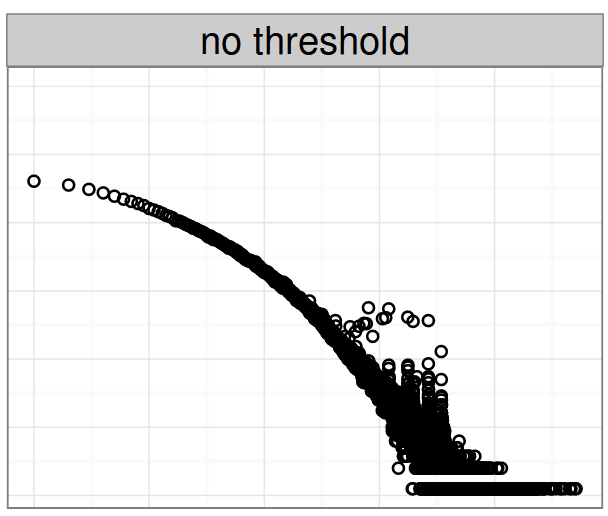
\includegraphics[width=\textwidth]{no-threshold-pdf.png}
\end{minipage}
\hfill
\begin{minipage}{0.32\linewidth}
	\centering
    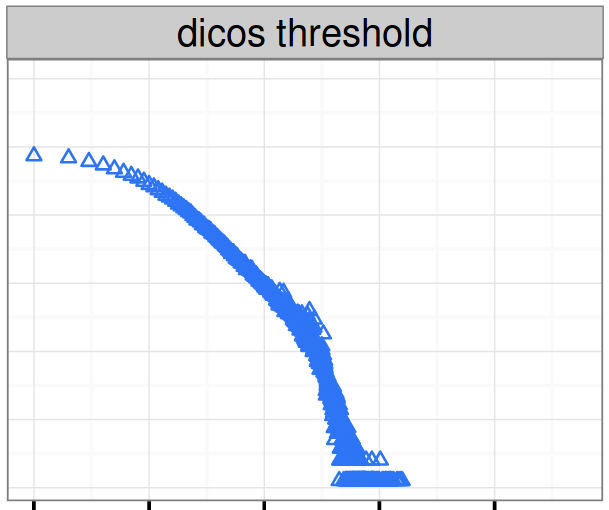
\includegraphics[width=\textwidth]{dicos-pdf.png}
\end{minipage}
\hfill
\begin{minipage}{0.32\linewidth}
	\centering
    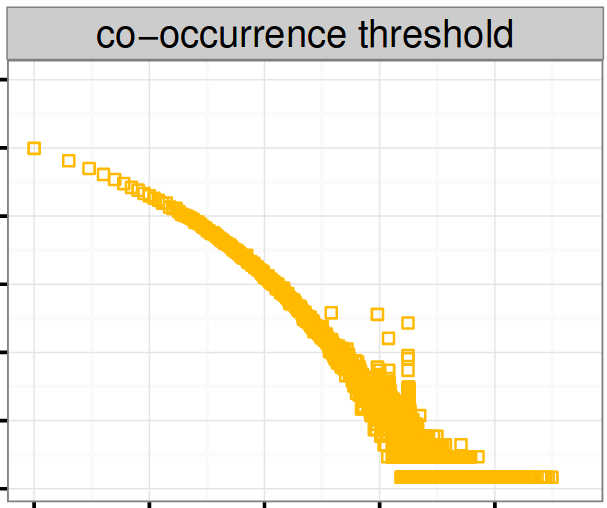
\includegraphics[width=\textwidth]{cooc-pdf.png}
\end{minipage}
\end{figure}

\begin{center}
The graph for \texttt{dicos} threshold suggests that this is a good measure of making the graph sparse, while not compromising a lot of particular details.
\end{center}
\end{frame}

\begin{frame}[fragile]
	\frametitle{\normalsize Effect of thresholding strategies on the resultant graphs {\small (contd..)}}
\vspace{-5mm}
\begin{itemize}
\item In a typical social network, it quite probably for people of similar ages / similar time periods to be connected to each other.
\item To check if the extracted network after threshold satisfies this temporal property at least approximately, the authors consider a difference in the birth date and death date (age) of adjacent nodes.
\item The distribution reveal that if this time span is greater than expected human lifespan, there is a dip in the probability.
\item The network obtained using \texttt{dicos} thresholding strategy favours shorter time-spans more than the networks obtained without thresholding and with a co-occurrence based thresholding.
\end{itemize}
\end{frame}

\begin{frame}[fragile]
	\frametitle{\normalsize Effect of thresholding strategies on the resultant graphs {\small (contd..)}}
\vspace{-5mm}
\begin{figure}
	\centering
    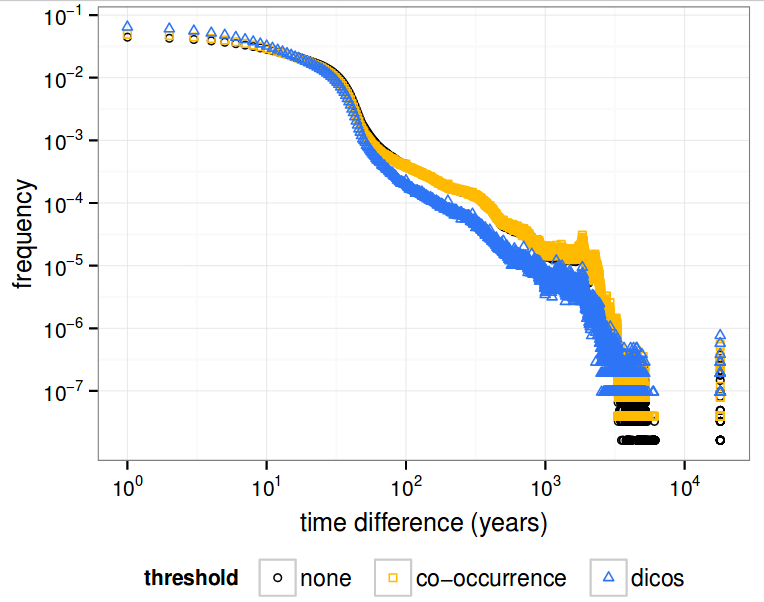
\includegraphics[width=0.7\textwidth]{time-span-pdf.png}
\end{figure}

\begin{center}
Note the time difference at the first elbow in the distribution, which is what is typical of a social network graph.
\end{center}
\end{frame}

\begin{frame}[fragile]
	\frametitle{Finding network centrality}
\vspace{-5mm}
\begin{itemize}
\item Around which entity is the network centered?
\item How influential is the entity?
\item These are the types of questions addressed by identifying network centrality.
\item This can be done a very similar way as \texttt{TF-IDF}, which captures popular words.
\item The PageRank centrality is used to find out the centrality of the network, which is this case is a group of people in the network.
\item There could be correlation between the top referenced persons and network centres.
\begin{itemize}
	\item There is much more to computing the network centres, which takes into account the lifespan of the person and various others factors arising from the graph itself, for instance the weight.
    \item PageRank is claimed to have called the people in the past to be more popular, but that is not what network centrality captures.
\end{itemize}
\end{itemize}
\end{frame}

\begin{frame}[fragile]
	\frametitle{Finding network centrality{\small (contd..)}}
\vspace{-5mm}
\begin{figure}
	\centering
    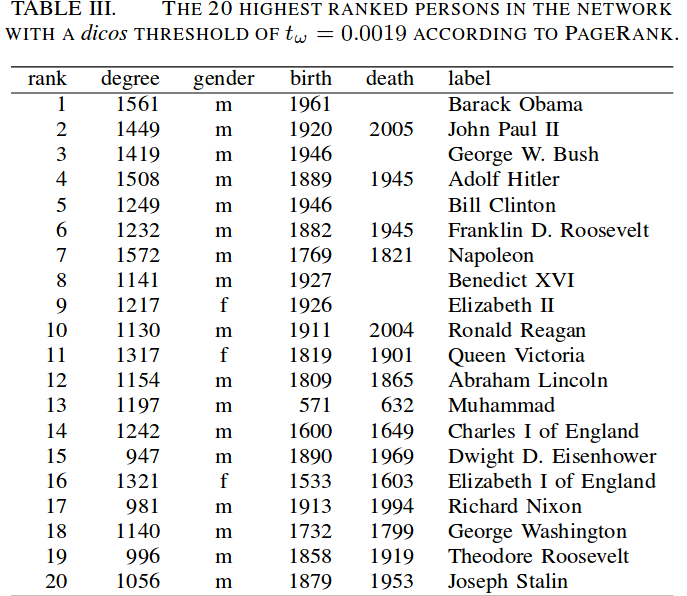
\includegraphics[width=0.7\linewidth]{network-centre.png}
\end{figure}
\end{frame}


\begin{frame}[fragile]
	\frametitle{Community Detection}
\vspace{-5mm}
\begin{itemize}
\item Detecting communities in networks is a well-studied problem.
\item This has led to multiple algorithms and analyses for networks.
\begin{itemize}
	\item These methods vary in speed, accuracy, applicability and so on.
\end{itemize}
\item One main problem in this network is the size of the network (~65 M edges, ~800K nodes). Traditional community detection algorithms will take a lot of time to complete, owing to the time complexities.
\item The authors consider from the survey and analysis conducted by Harenberg \textit{et al}, the SLPA (stabilized label propagation algorithm) as a community detection algorithm.
\end{itemize}
\end{frame}

\begin{frame}[fragile]
	\frametitle{\normalsize Stabilized Label Propagation Algorithm for this network}
\vspace{-7mm}
\begin{itemize}
\item Given a graph \(G = (V, E)\), the algorithm informally does this:
\begin{itemize}
	\item First assign a unique label to each node in the network
	\item In each subsequent step, for every node assign a label by performing a majority vote amongst the neighbours.
\end{itemize}
\item This algorithm could assign multiple label (note that you don't replace) to a given node, which causes two types of clustering : soft and hard.
\begin{itemize}
\item To obtain a soft clustering, assign a probability threshold \(p_{\text{thres}}\) so that a given node is not assigned to itself. Now the label for a node could be more than 1.
\item To obtain a hard clustering, assign the label of the most probable cluster.
\end{itemize}
\item The time complexity of SLPA is linear in \(|E|\), and linearly proportional to the number of time you want to propagate labels.
\end{itemize}
\end{frame}

\begin{frame}[fragile]
	\frametitle{Results of SLPA for this network}
\vspace{-10mm}
\begin{figure}
	\centering
    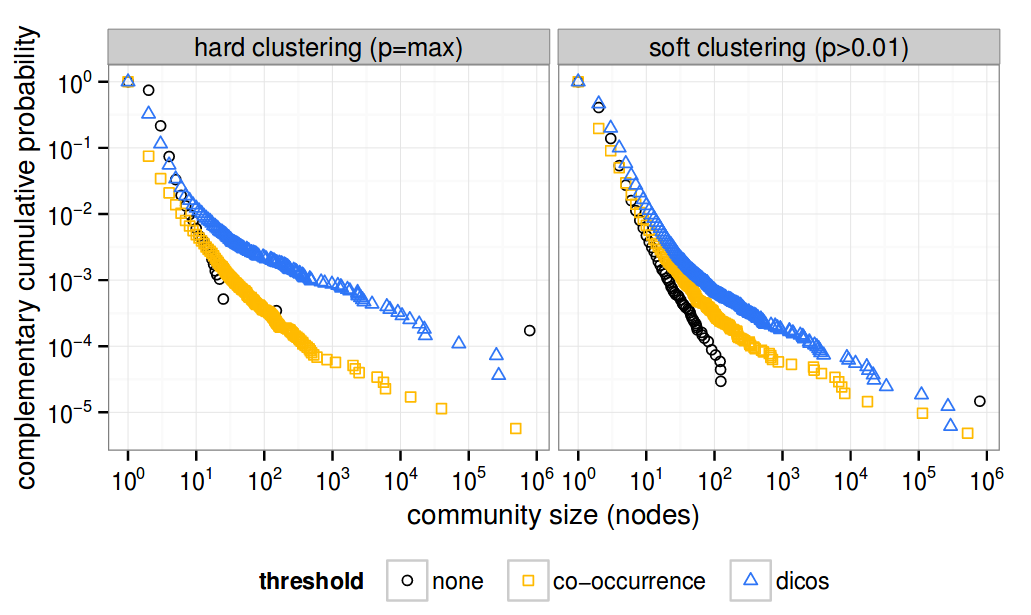
\includegraphics[width=0.8\linewidth]{comm-pdf.png}
\end{figure}
\begin{center}
Here the number of propagations made through the network is equal to 100. Note that the number of medium sized communities discovered is higher for the network obtained using \texttt{dicos} thresholding.
\end{center}
\end{frame}

\begin{frame}[fragile]
	\frametitle{\normalsize How good are my detected communities?}
\begin{itemize}
\item Identifying the effectiveness of community detection is not simple given the diversity of the data.
\begin{itemize}
	\item For instance, the authors states that Winston Churchill is part of 97 categories.
    \item There are \(\approx 5300\) people in only category, which may or may not be the same.
    \item The largest category is of size 438,500 - categorizing ``living people''.
\end{itemize}
\item How do you evaluate the algorithm?
\begin{itemize}
	\item Detour into set theory.
\end{itemize}
\end{itemize}
\end{frame}

\begin{frame}[fragile]
	\frametitle{Evaluation strategies}
\vspace{-15mm}
Define Precision (P), Recall (R) and F-Score (F) as:
\begin{itemize}
\item \(\displaystyle P = \frac{|\text{community} \cap \text{category}|}{|\text{community}|}\)
\item \(\displaystyle R = \frac{|\text{community} \cap \text{category}|}{|\text{category}|}\)
\item \(\displaystyle F = \frac{2PR}{P + R}\)
\end{itemize}
\begin{center}
Now, the authors compare an overall precision (across all communities) and between certain communities where \(n_{c} \in (10, 500)\), with different thresholding strategies (co-occurrence and \texttt{dicos}).
\end{center}
\end{frame}

\begin{frame}[fragile]
	\frametitle{Evaluation results and some discussion}
\vspace{-10mm}
\begin{figure}
	\centering
    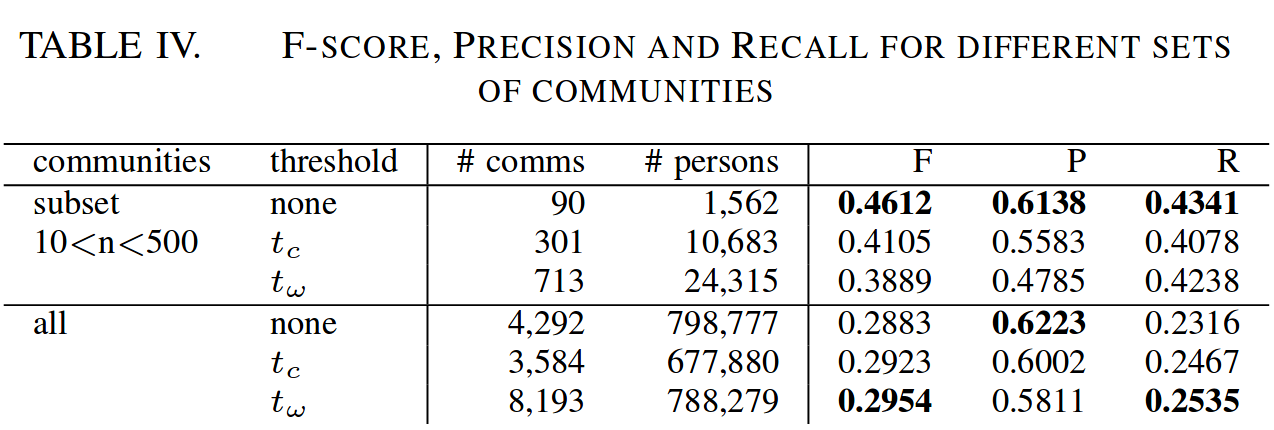
\includegraphics[width=0.75\linewidth]{table-eval.png}
\end{figure}
\begin{itemize}
\item This is entirely dependent on the policies of categorization which keeps changing.
\item This is also dependent on the scheme of thresholding used.
\item Hierarchical organization of categories in Wikipedia is a factor to be taken into consideration : to upto what level of hierarchy should we consider?
\item Semantically equivalent groups were identified, yet Wikipedia did not have that as a category.
\end{itemize}
\end{frame}

\begin{frame}[fragile]
	\frametitle{Conclusion}
\begin{itemize}
\item This paper provides an approach to get a person-centric network from Wikipedia.
\item Also gives a new weighting approach called \texttt{dicos} for weighting the relationship between two people
\item Show that a threshold based scheme is good for community detection and network centrality capturing tasks.
\end{itemize}
\end{frame}

\plain{Questions?}
\end{document}
